%% LyX 2.0.3 created this file.  For more info, see http://www.lyx.org/.
%% Do not edit unless you really know what you are doing.
\documentclass[12pt,english]{report}
\usepackage[T1]{fontenc}
\usepackage[latin9]{inputenc}
\usepackage{float}
\usepackage{calc}
\usepackage{amsthm}
\usepackage{amsmath}
\usepackage{setspace}

\makeatletter

%%%%%%%%%%%%%%%%%%%%%%%%%%%%%% LyX specific LaTeX commands.
\providecommand{\LyX}{L\kern-.1667em\lower.25em\hbox{Y}\kern-.125emX\@}
%% Because html converters don't know tabularnewline
\providecommand{\tabularnewline}{\\}
\floatstyle{ruled}
\newfloat{algorithm}{tbp}{loa}[chapter]
\providecommand{\algorithmname}{Algorithm}
\floatname{algorithm}{\protect\algorithmname}

%%%%%%%%%%%%%%%%%%%%%%%%%%%%%% Textclass specific LaTeX commands.
\usepackage{UTSAthesis}      
\usepackage{times}            
\usepackage{latexsym}

\newenvironment{ruledcenter}{%
  \begin{center}
  \rule{\textwidth}{1mm} } {%
  \rule{\textwidth}{1mm} 
  \end{center}}%


  \theoremstyle{definition}
  \newtheorem{defn}{\protect\definitionname}
\theoremstyle{plain}
\newtheorem{thm}{\protect\theoremname}

\newcommand{\basicEAP}{EAP_0^{1,1}}
\newcommand{\eapABAC}{EAP-ABAC}


\newcommand{\policyMachine}{Policy Machine}

\newcommand{\labac}{$LaBAC_{1}$}
\newcommand{\clabac}{$LaBAC_{0}$}
\newcommand{\hlabac}{$LaBAC_{H}$}
\newcommand{\slabac}{$LaBAC_{S}$}
\newcommand{\consLabac}{$LaBAC_{C}$}

\newcommand{\elabac}{$LaBAC_{E}^{1,1}$}

\newcommand{\clabacOneTwo}{$LaBAC_{0}$}
\newcommand{\hlabacOneTwo}{$LaBAC_{1}$}
\newcommand{\hlabacOneTwoTwo}{$LaBAC_{0}^{2,2}$}
\newcommand{\labacZeroTwoTwo}{$LaBAC_{0}^{2,2}$}
\newcommand{\labacOneOneOne}{$LaBAC_{1}$}
\newcommand{\labacZeroOneOne}{$LaBAC_{0}$}
\newcommand{\labacZeroMN}{$LaBAC_{0}^{m,n}$}
\newcommand{\abacAlpha}{ABAC_\alpha}
\newcommand{\hgabac}{HGABAC}
\newcommand{\uLabel}{uLabel}
\newcommand{\oLabel}{oLabel}

\newcommand{\uLabelOne}{uLabel_1}
\newcommand{\oLabelOne}{oLabel_1}
\newcommand{\uLabelTwo}{uLabel_2}
\newcommand{\oLabelTwo}{oLabel_2}
\newcommand{\canAddPolicy}{can\_manage\_policy}



%-- LaBAC new commands---

\newcommand{\lb}{ }
\newcommand{\OBJ}{O}
\newcommand{\objmem}{o}
\newcommand{\U}{U}
\newcommand{\umem}{u}
\newcommand{\amem}{a}
\newcommand{\A}{A}
\newcommand{\OL}{OL}
\newcommand{\UL}{UL}
\newcommand{\OLV}{OL}
\newcommand{\olvmem}{ol}
\newcommand{\ULV}{UL}
\newcommand{\ulvmem}{ul}
\newcommand{\OLA}{OLA}
\newcommand{\ULA}{ULA}
\newcommand{\OLH}{OLH}
\newcommand{\ULH}{ULH}

\newcommand{\Policy}{Policy}
\newcommand{\policy}{Policy}

\newcommand{\creator}{creator}

\newcommand{\odominate}{\succeq_{ol}}
\newcommand{\udominate}{\succeq_{ul}}

\newcommand{\allowedLabels}{allowed\_counter\_labels}
\newcommand{\restrictedTuples}{RestrictedTuples}



\newcommand{\oLabelH}{oLabel^*}
\newcommand{\uLabelH}{uLabel^*}
\newcommand{\impliedPolicy}{ImpliedPolicy}
\newcommand{\effectivePolicy}{Effective\_policy}
\newcommand{\policyBound}{ValidTuples}
\newcommand{\sessionLabels}{s\_labels}
\newcommand{\CircuitSAT}{CircuitSAT}
\newcommand{\maxPolicy}{|policy|_{max}}
\newcommand{\maxPolicySet}{|\policy|_{max}}
\newcommand{\request}{is\_authorized}



\newcommand{\requestContext}{ReqContext}
\newcommand{\reviewFunction}{R}

\newcommand{\sABAC}{$ABAC_s$}

\newcommand{\twoSortedRBAC}{2-sorted-RBAC}
\newcommand{\properRole}{R^+}
\newcommand{\properRoleHierarchy}{R^+H}
\newcommand{\demarcationHierarchy}{D^+H}
\newcommand{\roles}{R^+}
\newcommand{\RH}{R^+H}
\newcommand{\demarcation}{D^+}
\newcommand{\DeH}{D^+H}
\newcommand{\PD}{PD^+}
\newcommand{\SR}{SR^+}

%----------------Session / object creation functions--------------%
\newcommand{\createSession}{create\_session}
\newcommand{\deleteSession}{delete\_session}
\newcommand{\assignValues}{assign\_values}
\newcommand{\removeValues}{remove\_values}
\newcommand{\createReq}{session^+}
\newcommand{\removeReq}{session^-}
\newcommand{\sessionOL}{session}
\newcommand{\createObject}{create\_object}
\newcommand{\updateObject}{update\_OL\_values}
\newcommand{\assignLabels}{assign\_OL\_values}
\newcommand{\removeLabels}{remove\_OL\_values}

\newcommand{\createUser}{create\_user}
\newcommand{\assignULLabels}{assign\_UL\_values}
\newcommand{\removeULLabels}{remove\_UL\_values}

%-------------Policy Machine Command--------------------%
\newcommand{\pmMini}{PM_{mini}}
\newcommand{\assignment}{ASSIGN}
\newcommand{\assignmentPlus}{\assignment^+}
\newcommand{\assignmentStar}{\assignment^*}
\newcommand{\assignmentOOA}{\assignment_{ooa}}
\newcommand{\assignmentUUA}{\assignment_{uua}}
\newcommand{\assignmentOAOA}{\assignment_{oaoa}}
\newcommand{\assignmentUAUA}{\assignment_{uaua}}
\newcommand{\assignmentATPC}{\assignment_{atpc}}
\newcommand{\association}{ASSOCIATION}
\newcommand{\associationPolicy}{\association_{policy}}
\newcommand{\decisionFunction}{allow\_resource\_request}
\newcommand{\allAssignment}{ASSIGN}
\newcommand{\allAssociation}{ASSOC}
\newcommand{\peAssoc}{PC\_ASSOC}
\newcommand{\peAssign}{PC\_ASSIGN}
\newcommand{\assignmentLabac}{\assignment}
 \newcommand{\denom}{\empty}
 \newcommand{\suffix}{\empty}
 \newcommand{\suffixTwo}{\empty}
 \renewcommand{\suffix}{m,n}
 \newcommand{\suffixT}{1,1}
 
\newcommand{\PM}{\textit{PM}}
\newcommand{\LAP}{\textit{LAP}}
\newcommand{\EAP}{\textit{EAP}}
\newcommand{\TL}{\textit{TL}}
%
\newcommand{\userLabel}[1]{uLabel_{#1}}
\newcommand{\objectLabel}[1]{oLabel_{#1}}
%\newcommand{\UL}[1]{UL_#1}
%\newcommand{\OL}[1]{OL_#1}
%\newcommand{\userLabelOne}{$uLabel_1$}
%
%
%%---------EP-ABAC Models---------------%
\newcommand{\EPModels}{$EAP$-$ABAC$}
\newcommand{\EPZeroOneOne}{$EP_{0}$-$ABAC^{1,1}$}
\newcommand{\EPHOneOne}{$EP_{H}$-$ABAC^{1,1}$}
\newcommand{\EPSOneOne}{$EP_{S}$-$ABAC^{1,1}$}
\newcommand{\EPPMOneOne}{$EP_{\pm}$-$ABAC^{1,1}$}
\newcommand{\EPOneOneModels}{$EAP$-$ABAC_{1,1}$}
\newcommand{\EPMNModels}{$EP$-$ABAC^{m,n}$}
%
%\newcommand{\EPZeroOneOne}{\clabac}
%\newcommand{\EPHOneOne}{\hlabac}
%\newcommand{\EPSOneOne}{\slabac}
%\newcommand{\EPPMOneOne}{\npLabac}
%\newcommand{\EPOneOneModels}{$EAP$-$ABAC_{1,1}$}
\newcommand{\EPMNModel}{$EAP$-$ABAC_{m,n}$}
%
%
\newcommand{\LPModels}{$LAP$-$ABAC$}
\newcommand{\LPOneOne}{$LAP$-$ABAC_{1,1}$}
\newcommand{\LPMN}{$LAP$-$ABAC_{m,n}$}
\newcommand{\pmlabac}{$LaBAC_{\pm}^{1,1}$}
%
%% ---------------Other models-----------------
%\newcommand{\abacAlpha}{ABAC_\alpha}
%\newcommand{\hgabac}{$HGABAC$}
%\newcommand{\twoSortedRBAC}{2-sorted-RBAC}
%
%% ------------Higher Level LABAC---------------
%
%\newcommand{\labacOneTwoTwo}{$LaBAC_{1}^{2,2}$}
%\newcommand{\labacOneOneOne}{$LaBAC_{1}^{1,1}$}
%\newcommand{\labacOneMN}{$LaBAC_{1}^{m,n}$}
%\newcommand{\labacZeroMN}{$LaBAC_{0}^{m,n}$}
%\newcommand{\setLabac}{$LaBAC_{S}^{1,1}$}
%
%\newcommand{\labacNPMN}{$LaBAC_{\pm}^{m,n}$}
%\newcommand{\abacOneOne}{$LP$-$ABAC^{1,1}$}
%\newcommand{\labacOneOne}{$LaBAC^{1,1}$}
%
%%--------- LaBAC Names -----
%\newcommand{\labac}{$LaBAC$}
%\newcommand{\clabac}{$LaBAC_{0}^{1,1}$}
%\newcommand{\hlabac}{$LaBAC_{H}^{1,1}$}
%\newcommand{\slabac}{$LaBAC_{S}^{1,1}$}
%\newcommand{\npLabac}{$LaBAC_{\pm}^{1,1}$}
%\newcommand{\consLabac}{$LaBAC_{C}^{1,1}$}
%\newcommand{\elabac}{$LaBAC_{E}^{1,1}$}
%\newcommand{\labacOneOneFamily}{$LaBAC^{1,1}$}
%
%
%%------------LaBAC administrative ops-------------%
%\newcommand{\policyReview}{policy\_review}
%
%
%%-------------------- LaBAC Components-----------------
%\newcommand{\uLabel}{uLabel}
%\newcommand{\oLabel}{oLabel}
%\newcommand{\uLabelOne}{uLabel_1}
%\newcommand{\oLabelOne}{oLabel_1}
%\newcommand{\uLabelTwo}{uLabel_2}
%\newcommand{\oLabelTwo}{oLabel_2}
%\newcommand{\canAddPolicy}{can\_manage\_policy}
%\newcommand{\lb}{ }
%\newcommand{\OBJ}{O}
%\newcommand{\objmem}{o}
%\newcommand{\U}{U}
%\newcommand{\umem}{u}
%\newcommand{\amem}{a}
%\newcommand{\A}{A}
%
%\newcommand{\OLV}{OL}
%\newcommand{\olvmem}{ol}
%\newcommand{\ULV}{UL}
%\newcommand{\ulvmem}{ul}
%\newcommand{\OLA}{OLA}
%\newcommand{\ULA}{ULA}
%\newcommand{\OLH}{OLH}
%\newcommand{\ULH}{ULH}
%
%\newcommand{\policy}{Policy}
%\newcommand{\odominate}{\succeq_{ol}}
%\newcommand{\udominate}{\succeq_{ul}}
%\newcommand{\impliedPolicy}{Implied\_policy}
%\newcommand{\effectivePolicy}{Effective\_policy}
%\newcommand{\policyBound}{ValidPolicy}
%
%\newcommand{\maxPolicy}{|policy|_{max}}
%\newcommand{\maxPolicySet}{|\policy|_{max}}
%\newcommand{\request}{is\_authorized}
%
%
%% -------------session command------------
%\newcommand{\addSessionLabels}{add\_session\_labels}
%\newcommand{\removeSessionLabels}{remove\_session\_labels}
%\newcommand{\addSessionValues}{add\_session\_values}
%\newcommand{\removeSessionValues}{remove\_session\_values}
%\newcommand{\createSession}{create\_session}
%\newcommand{\deleteSession}{delete\_session}
%\newcommand{\createSubject}{create\_subject}
%\newcommand{\deleteSubject}{delete\_subject}
%\newcommand{\assignValues}{assign\_values}
%\newcommand{\removeValues}{remove\_values}
%
%%------------------ABAC^11 commands--------------
%
\newcommand{\UAV}[1]{\textit{UAV}_{#1}}
\newcommand{\OAV}[1]{\textit{OAV}_{#1}}
\newcommand{\ua}[1]{ua_{#1}}
\newcommand{\sa}[1]{sa_{#1}}
\newcommand{\oa}[1]{oa_{#1}}
\newcommand{\subCreator}{creator}
\newcommand{\uLabelP}[1]{\uLabel_{#1}}
\newcommand{\oLabelP}[1]{\oLabel_{#1}}
\newcommand{\ULS}[1]{ULS_{#1}}
\newcommand{\OLS}[1]{OLS_{#1}}
\newcommand{\val}[1]{\textit{Val}_{#1}}
\newcommand{\uVal}[1]{\textit{uVal}_{#1}}
\newcommand{\oVal}[1]{\textit{oVal}_{#1}}
\newcommand{\sessionLabelsP}[1]{\sessionLabels_{#1}}


%---------------ABAC, labac equivalence commands------------

\newcommand{\isAuthorized}{is\_authorized}
\newcommand{\GammaLabac}{\Gamma^{L}}
\newcommand{\gammaLabac}{\gamma^{L}}
\newcommand{\GammaA}{\Gamma^{A}}
\newcommand{\gammaA}{\gamma^{A}}
\newcommand{\GammaB}{\Gamma^{L}}
\newcommand{\gammaB}{\gamma^{L}}
\newcommand{\QLabac}{Q^{L}}
\newcommand{\qLabac}{q^{L}}
\newcommand{\QA}{Q^{A}}
\newcommand{\qA}{q^{A}}
\newcommand{\QB}{Q^{L}}
\newcommand{\qB}{q^{L}}
\newcommand{\qs}{q_s^{L}}
\newcommand{\qsa}{q_s^{A}}

\newcommand{\vdashA}{\vdash^{A}}
\newcommand{\vdashB}{\vdash^{L}}
\newcommand{\vdashLabac}{\vdash^{L}}
\newcommand{\GammaABAC}{\Gamma^{A}}
\newcommand{\gammaABAC}{\gamma^{A}}
\newcommand{\QABAC}{Q^{A}}
\newcommand{\qABAC}{q^{A}}
\newcommand{\vdashABAC}{\vdash^{A}}
\newcommand{\PABAC}{P^A}
\newcommand{\PLabac}{P^L}
\newcommand{\qal}{q_{aij}^L}
\newcommand{\qaa}{q_{aij}^A}
\newcommand{\ulpm}{UL_{\pm} }
\newcommand{\olpm}{OL_{\pm} }
\newcommand{\ulsubset}{UL_i}
\newcommand{\olsubset}{OL_j}
\newcommand{\gammaStartLabac}{\gamma_{0}^{L}}
\newcommand{\gammaStartABAC}{\gamma_{0}^{A}}
\newcommand{\gammaKLabac}{\gamma_{k}^{L}}
\newcommand{\gammaKABAC}{\gamma_{k}^{A}}

\newcommand{\mapping}{\overset{*}{\longmapsto_\psi}}
\newcommand{\mappingABAC}{\overset{*}{\longmapsto_{\psi_{A}}}}

%--------Tripli Commands ---------------
\newcommand{\mygamma}[2]{\gamma_{#1}^{#2}}
\newcommand{\myGamma}[1]{\Gamma^{#1}}
\newcommand{\mylongmapsto}[1]{\overset{*}{\longmapsto_#1}}
%\newcommand{\myVdash}{1}{\vdash^{#1}}
\newcommand{\myvdash}[1]{\vdash^{#1}}

\newcommand{\myq}[2]{q_{#1}^{#2}}
\newcommand{\myQ}[1]{Q^{#1}}
\newcommand{\myPSI}[1]{\Psi^{#1}}


%----------policy review functions---------


\newcommand{\subsetUL}{UL_s}
\newcommand{\subsetOL}{OL_s}
\newcommand{\setULs}{2^{UL}}
\newcommand{\setOLs}{2^{OL}}

%---------Tripli equivalence functions----------
\newcommand{\smallGamma}[1]{\gamma^{#1}}
\newcommand{\bigGamma}[1]{\Gamma^{#1}}
\newcommand{\smallQ}[1]{q_{s}^{#1}}
\newcommand{\bigQ}[1]{Q^{#1}}
\newcommand{\bigVdash}[1]{\vdash^{#1}}
\newcommand{\smallPsi}[1]{\psi^{#1}}
\newcommand{\bigPsi}[1]{\Psi^{#1}}

\newcommand{\curModelSymbol}{Z}
\newcommand{\manager}{mng}
\newcommand{\atom}{\textit{AtOM}}
%\newcommand{\labac}{LaBAC}
\newcommand{\eapabac}{EAP-ABAC}

%\newcommand{\uLabel}{uLabel}
%\newcommand{\oLabel}{sLabel}
%\newcommand{\request}{is\_authorized}
\newcommand{\policyTuples}{\textit{Policy-tuples}}
%\newcommand{\udominate}{\succeq_{ul}}
%\newcommand{\odominate}{\succeq_{sl}}
%\newcommand{\VTH}{\succeq_{t}}
\newcommand{\DMH}{\succeq_{d}}
\newcommand{\JEH}{\succeq_{j}}
\newcommand{\labelAssignment}{LabelAssignments}
\newcommand{\canAccess}{can\_access}
\newcommand{\matchingElements}{MatchingElements}
\newcommand{\exactMatch}{\textit{exact-match}}
\newcommand{\partialMatch}{\textit{partial-match}}
\newcommand{\match}{\textit{direct-containment}}

\newcommand{\oneLevelUP}{\textit{one-level-up}}
\newcommand{\cascadeUP}{\textit{cascade-up}}
\newcommand{\oneLevelDown}{\textit{one-level-down}}
\newcommand{\cascadeDown}{\textit{cascade-down}}


\newcommand{\noProp}{\textit{no-prop}}
\newcommand{\unrestrictedLabeling}{\textit{unrestricted-labeling}}
\newcommand{\restrictedLabeling}{\textit{restricted-labeling}}
\newcommand{\defaultLabeling}{\textit{default-labeling}}

\newcommand{\reForEmail}{RE\_EMAIL}
\newcommand{\reCreditCard}{RE\_CREDIT\_CARD}
\newcommand{\reSSN}{RE\_SSN}
%%%%%%%%%%%%%%%%%%%%%%%%%%%%%% User specified LaTeX commands.
\usepackage{epsfig}          
\usepackage{setspace}         
\usepackage{lscape}
\usepackage{graphicx}
\usepackage{cite}
\usepackage{algorithm}
\usepackage[noend]{algorithmic}
\usepackage{xspace}
\usepackage{enumerate}
\usepackage{array} 
\usepackage{color}
\usepackage{cases}
\usepackage{amsfonts}
\usepackage{xcolor}
\usepackage{url}

%%%%-----------------Packages from ABAC16 papers------------------%%%%%%%%

\usepackage{amsmath}
\usepackage{listings}
\usepackage{underscore}
\usepackage{enumitem}
\usepackage{etoolbox}
\usepackage{graphicx}
\usepackage{booktabs}
%\usepackage{algorithm}
%\usepackage{algpseudocode}
\usepackage{pifont}
\usepackage{lipsum,multicol}
\usepackage[T1]{fontenc}
\usepackage{epstopdf}
\epstopdfsetup{outdir=./}
\usepackage{amssymb}
\usepackage{float}
\usepackage{flushend}
\usepackage{caption}
%\usepackage{hyperref}

%%%--------------ENd ABAC16 package imports-----------------%%%%

\@ifundefined{showcaptionsetup}{}{%
 \PassOptionsToPackage{caption=false}{subfig}}
\usepackage{subfig}
\makeatother

\usepackage{babel}
  \providecommand{\definitionname}{Definition}
\providecommand{\theoremname}{Theorem}

\begin{document}



\committee{Prof. Ravi Sandhu, Ph.D.}{Prof. Jianwei Niu, Ph.D.}{Prof. Gregory White, Ph.D.}{Prof. Palden Lama, Ph.D.}{Prof. Ram Krishnan, Ph.D. }


\informationitems{Doctor of Philosophy in Computer Science}{Ph.D.}{M.Sc.}{Department of Computer Science}{College of Sciences}{May}{2017}


%\thesiscopyright{Copyright 2017 Prosunjit Biswas\\All rights reserved. }


\dedication{\emph{To my father Gobinda Chandra Biswas and mother Monmila Biswas who have always inspired me through their noble qualities and wisdom.}}


\title{\textbf{Enumerated Authorization Policy ABAC Models:
Expressive Power and Enforcement
} 
}


\author{Prosunjit Biswas}
\maketitle
\begin{acknowledgements}
First of all, I would like to thank Kevin Xu Su for creating an earlier
version of the \LaTeX{} style, Lijie Zhang for using an earlier version
of this package to write her dissertation and to provide feedback. 

I would also like to thank the UTSA Graduate School for reviewing
the outcome of this template document and correction of formatting
errors. 

(Notice: If any part of the thesis/dissertation has been published
before, the following two paragraphs should be included without alteration).

\begin{singlespace}
\emph{This Masters Thesis/Recital Document or Doctoral Dissertation
was produced in accordance with guidelines which permit the inclusion
as part of the Masters Thesis/Recital Document or Doctoral Dissertation
the text of an original paper, or papers, submitted for publication.
The Masters Thesis/Recital Document or Doctoral Dissertation must
still conform to all other requirements explained in the Guide for
the Preparation of a Masters Thesis/Recital Document or Doctoral Dissertation
at The University of Texas at San Antonio. It must include a comprehensive
abstract, a full introduction and literature review, and a final overall
conclusion. Additional material (procedural and design data as well
as descriptions of equipment) must be provided in sufficient detail
to allow a clear and precise judgment to be made of the importance
and originality of the research reported. }

\emph{It is acceptable for this Masters Thesis/Recital Document or
Doctoral Dissertation to include as chapters authentic copies of papers
already published, provided these meet type size, margin, and legibility
requirements. In such cases, connecting texts, which provide logical
bridges between different manuscripts, are mandatory. Where the student
is not the sole author of a manuscript, the student is required to
make an explicit statement in the introductory material to that manuscript
describing the students contribution to the work and acknowledging
the contribution of the other author(s). The signatures of the Supervising
Committee which precede all other material in the Masters Thesis/Recital
Document or Doctoral Dissertation attest to the accuracy of this statement.}\end{singlespace}
\end{acknowledgements}

\begin{abstract}
Attribute Based Access Control (ABAC) has gained considerable attention from businesses, academia and standards bodies (e.g. NIST  and NCCOE ) in recent years. ABAC uses attributes on users, objects and possibly other entities (e.g. context/environment), and specifies rules using these attributes to assert who can have which access permissions (e.g. read/write) on which objects.  Although ABAC concepts have been around for over two decades, there remains a lack of well-accepted ABAC models.  Recently there has been a resurgence of interest in ABAC due to continued dissatisfaction with the traditional models---notably Role Based Access Control (RBAC), Discretionary Access Control (DAC), and Lattice Based Access Control (LBAC).

There are two major techniques stated in the literature for specifying authorization policies in Attribute Based Access Control. The more conventional approach is to define policies by using logical formulas involving attribute values. The alternate technique for expressing policies is by enumeration. While considerable work has been done for the former approach, the later is comparatively less studied.  

%There remains many fundamental research problem to investigate, such as how to enumerate an authorization policy, how an enumerated authorization policy ABAC model should look like,  how enumerated policy is related to logical-formula policy and so on. 

In this dissertation, we conduct a systematic study of Enumerated Authorization Policy (EAP) for ABAC. We have developed a representative, simple EAP ABAC model---EAP-ABAC$^{1,1}$. For the sake of clarity and emphasis on different elements of the model, we present EAP-ABAC$^{1,1}$ as a family of models. We have investigated how the defined models are comparable to other existing EAP models. We also demonstrate capability of the defined models by configuring traditional LBAC and RBAC models in them. 

We compare theoretical expressive power of EAP based ABAC models to logical-formula authorization policy ABAC models. In this regard, we present a finite-attribute, finite-domain ABAC model for enumerated authorization policies and investigate its relationship with logical-formula authorization policy ABAC models in the finite domain. We show that these models (EAP-ABAC and LAP-ABAC) are equivalent in their theoretical expressive power. We respectively show that single and multi-attribute ABAC models are equally expressive.

As proof-of-concepts, we demonstrate how EAP ABAC models can be enforced in different application contexts. We have designed an enhanced EAP-ABAC$^{1,1}$ model to protect JSON documents. While most of the existing XML protection model consider only hierarchical structure of underlying data, we additionally identify two more inherent characteristics of data--- semantical association and scatteredness and consider them in the design. Finally, we have outlined how EAP-ABAC$^{1,1}$ can be used in OpenStack Swift to enhance its ``all/no access'' paradigm to ``policy-based selective access''.



\end{abstract}


\pageone{}

\section{Introduction}

Access control has been a major component in enforcing security and privacy requirements of information and resources with respect to unauthorized access. While many access control models have been proposed only three, viz., DAC, MAC and RBAC, have received meaningful practical deployment. DAC (Discretionary Access Control) \cite{sandhu1994access} allows resource owners to retain control on their resources by specifying who can or cannot access certain resources. To address inherent limitations of DAC such as trojan horses, MAC (Mandatory Access Control) \cite{sandhu1994access}  has been proposed which mandates access to resources by pre-specified system policies. While both of these two models are based on fixed and predetermined policies, RBAC (Role Based Access Control) \cite{rbac} is a policy neutral, flexible and administrative friendly model.  Notably RBAC is capable of enforcing both DAC and MAC.  MAC is also commonly referred to as LBAC (Lattice-Based Access Control).

Attribute Based Access Control (ABAC) has gained considerable attention from businesses, academia and standard bodies (NIST \cite{nist-abac-draft} and NCCOE \cite{nccoe-abac-draft}) in recent years. ABAC uses attributes on users, objects and possibly other entities (e.g. context/environment) and specifies rules using these attributes to assert who can have which access permissions (e.g. read/write) on which objects.  Although ABAC concepts have been around for over two decades there remains a lack of well-accepted ABAC models.  Recently there has been a resurgence of interest in ABAC due to continued dissatisfaction with the three traditional models, particularly the limitations of RBAC.

%On the other hand, researchers and practitioners have long recognized essence of  attributes (user attributes, object attributes and context/environment attributes) in authentication and/or authorization decisions. For example, X.500 and X.509 \cite{xfiveonine}, LDAP \cite{ldap} or XACML \cite{xacml} are available for a long time which use attributes for either authentication or authorization decision. Some advantages of attributes in the authorization decision include following.

%Besides these models, researchers and practitioners have long recognized essence of  attributes (user attributes, object attributes and context/environment attributes) in authentication and/or authorization decisions. For example, X.500 and X.509 \cite{xfiveonine}, LDAP \cite{ldap} or XACML \cite{xacml} are familiar practitioner standard in this line available for a long time. The motivation of using attributes along with identities is long-standing. Attributes over identities are convenient in the following ways.

%\begin{itemize}
	%\item \emph{Hard to know user's real identity in a Open Environment: } In order to use identities, user's real identity has to be known beforehand. Often time, it is not possible to know the real identity of a user, specially when users come from a open environment like the Internet.
	
	%\item \emph{Hard to manage access control decision in large scale using Identity:} Using identities to specify access control decision, soon become infeasible when there are large number of users or objects to manage. On the other hand, as many users or objects can be specified using smaller set of attributes, they  are more preferable  in large distributed environment.
	
	%\item \emph{Anonymity or partial Identity:} Some times it is not required or even desirable to provide access control without knowing the real identity of a user. For example, in case of a digital library it may be enough to know some of the user attributes like membership or affiliation. On the other hand, for eligibility requirement of buying an alcoholic beverage, the age attribute may suffice without revealing the real identity.
	
	%\item \emph{Richer model for business function or logic in the authorization process:} Role, role hierarchy, role-based constraint easily capture some of the business function or logic of an organization related to role or job position in the organization. But in order to express business requirements in a more coherent way, it requires support for additional attributes.
	
%\end{itemize}



%Motivated by these requirements, various models have been proposed that accommodate attributes with traditional RBAC model \cite{rbac-with-attribute1, kuhn2010adding}. Another line of work is toward defining  a standalone model for Attribute Based Access Control (ABAC).

To demonstrate expressive power and flexibility, several ABAC models including  \cite{abacAlpha,hgabac,abac-for-web-service} have been proposed in past few years. These models adopt the conventional approach of designing attribute based rules/policies as logical formulas. Using logical formulas to grant or deny access is convenient because of the following reasons.

\begin{itemize}
	\item \emph{Simple and easy:} Creating a new rule for granting access is simple. It does not involve upfront cost like engineering roles in case of RBAC.
	
	\item \emph{Flexible:} Rules are easy to succinctly specify even complex policies. There is no limit on how many attributes can be used in a rule or how complex the language be to specify the rule. Given a required set of attributes, and a computational language, ABAC policy is only limited to what the language can express \cite{nist-abac-draft}.
\end{itemize}

Interestingly, designing a rich computational language to define attribute-based rules makes policy update or policy review an NP-complete or even undecidable problem. For example, authorization policies in many existing ABAC models including \cite{abacAlpha, hgabac, abac-for-web-service} are expressed  in propositional logic. Reviewing policy in these models (which may simply ask, for a given policy  which (attribute, value) pairs evaluate the policy to be true) is similar to the satisfiability problem in propositional logic which is NP-complete. Likewise review for policies specified in first-order logic is undecidable.

Another method for specifying attribute-based policies is by enumeration. Policy Machine \cite{policy-machine} and \twoSortedRBAC{} \cite{two-sorted-rbac} fall into this category. Enumerated policies  can also be very expressive. Ferraiolo et al \cite{policy-machine} show configuration of LBAC, DAC and RBAC in Policy Machine using enumerated policies.  Moreover, updating or reviewing an enumerated policy is inherently simple (polynomial time) because of its simple structure.  It should be noted that the size of an enumerated policy may be exponential relative to a succinct formula which expresses the same policy.  Thus there is a trade-off between these two methods for specifying policies.

In this paper, we present an ABAC model named Label-Based Access Control (LaBAC). In LaBAC, users are assigned a single label named $\uLabel$ and objects are assigned a single label named $\oLabel$. For a particular action, a policy in LaBAC is an enumeration using $\uLabel$ and $\oLabel$ values.

Labels ($\uLabel$ and $\oLabel$) in LaBAC are special types of attributes. While semantics of attributes in general are open-ended, labels have very specific semantics. For example, in general attributes can be set valued (e.g. roles) or atomic valued (e.g. age). Values of an attribute can be assigned by administrators (e.g. roles), derived from other attributes (e.g. membership type), self asserted (e.g. date of birth),  system specified (e.g. time) and so on. Moreover, values can be ordered or unordered.  On the other  hand, labels are specifically defined to be set valued, values are partially ordered and are only assigned by administrators. Intentionally, we use abstract names for labels---$\uLabel$ and $\oLabel$.  In an actual instance of LaBAC, labels can be given more appropriate names. For example, roles or clearance for $\uLabel$ and classification or sensitivity for $\oLabel$.

%In this paper, we represent LaBAC as a family of models---starting from the basic model, \clabac{} to the most advanced model, \labacOneOneOne{}.  In \hlabac{}, we add label hierarchies to \clabac{} while in \consLabac{} we add additional machinery to express constraints using labels. Finally, \labacOneOneOne{} combines all three models.

We analyze the expressive power of LaBAC with respect to other enumerative models. We also show that LaBAC can be viewed as a simple instance of Policy Machine (PM).  While, PM is more general and complex by covering other interesting aspects of access control, LaBAC is more scoped regarding development and progress towards ABAC models. On the other hand, we show equivalence of LaBAC and \twoSortedRBAC{} with respect to theoretical expressive power. Finally, we show flexibility of LaBAC by configuring traditional models (LBAC \cite{lbac} and RBAC\cite{rbac}) in it.

Rest of the paper is organized as follows. In Section \ref{sec:background}, we briefly discuss logic-based policy and enumerated policy along with a review of related literature. Section \ref{sec:model} presents a family of LaBAC models. We show the equivalence of LaBAC and \twoSortedRBAC{} in Section \ref{sec:equivalence}. Section \ref{sec:configuration} presents configuration of tradition RBAC and LBAC policy in LaBAC. We express LaBAC as a simple instance of Policy Machine in Section \ref{sec:pm}. Finally, Section \ref{sec:conclusion} concludes the paper.

%   which adopts the enumerated style for expressing authorization policies. LaBAC can  be viewed as a simple instance of Policy Machine (PM). LaBAC uses one user attribute ($\uLabel$) and one object attribute ($\oLabel$) and a authorization policy in LaBAC for an action is an enumeration using these two attributes. 


\section{Authorization policy representation}

\label{sec:background}
In this section, we discuss two types of authorization policies - logical-formula and enumerated policy wrt finite domain attributes based on the assumption of the finiteness of attribute values. 
\subsubsection{Finite domain ABAC}
%\textbf{Finite domain ABAC model}
	\section{Assumption of Finite Domains}
\subsection{Finite policies for Finite domain ABAC}

\textbf{Theorm 1:} \\
For L boolean variables at most $2^{2^L}$ distinct boolean expression can be defined over logical AND, OR and NOT operators. 

\textbf{Theorm 2:} \\
Let UA be the set of user attributes, OA be the set of object attributes and $A=UA \cup OA$. For an attribute $a \in A$, let $R(a)$ denote co-domain or range of the attribute. Further $OPS$ be the set of all comparison operators that compares user/object attribute with other attribute values or constant values. The maximum number of boolean variable (expression of the form (value op value) ) that can be defined comparing attribute values are $|A| \times |OP| \times \sum_{a \in A} R(a)$
	%\subsection{Enumerated \& logical-formula authorization policy}

\vspace{-.5em}
%\textbf{Logical-formula authorization policy}
\subsubsection{Logical-formula authorization policy}
Logical-formula authorization policy (\LAP{}) can be defined as a boolean expression consisting of subexpressions connected with logical operators (for example, $\land, \lor, \lnot$ and so on ) where each subexpression compares attribute values with other attribute or constant values. The language for \LAP{} usually supports a large set of logical and relational operators. A \LAP{} grants a user request for exercising certain action on an object if attributes of the requesting user and requested object evaluate the formula true. $Auth_{read} \equiv clearance(u) \succeq classification(o)$ is an example of  logical-formula authorization policy which allows a user to read an object if the user's clearance dominates classification of the object.

\LAP{}s are usually expressed in propositional logic. Examples of  \LPModels{} models  include \cite{abacAlpha,hgabac,abac-ws,abac-for-web-service}.  Flexibility of these models have been demonstrated by configuring conventional DAC\cite{dac}, MAC\cite{lbac} and RBAC \cite{rbac} policies in it. It has been shown  \cite{labac} that policy review in  \LPModels{} is equivalent to the satisfiability problem  which is NP-complete for propositional logic. 
\vspace{-1em}
%in proposition logic (or in first-order logic if LAPs are expressed in it) which makes the complexity of reviewing policies NP-complete in \LPModels{} models.


%\textbf{Enumerated authorization policy}
\subsubsection{Enumerated authorization policy}
	An enumerated authorization policy (\EAP{}) consists of a set of  tuples.  Each tuple \textit{(UAVals, OAVals)} grants privileges to a set of users  to exercise an action on a set of objects identified by the user and object attribute values \textit{UAVals} and \textit{OAVals} respectively. In an EAP, each tuple is distinct and grants privileges independently. Both  UAVals{} and OAVals{} can be atomic valued or set valued. (\textit{\manager, TS}) and (\textit{\{\manager, dir\}, \{TS,H\}}) are example of atomic and set valued tuples respectively. 
	
Usefulness of \EAP{}s have been demonstrated in the literature. For example, \textit{Policy Machine (PM)} \cite{policy-machine} and \labac{} \cite{labac} show flexibility of \EAP{}s by their ability to configure traditional models. 


%For example, in Policy Machine (PM) \cite{policy-machine}, Ferraiolo et. al define attribute based enumerated policies using one user attribute, one object attribute and a set of actions. PM also shows how to configure traditional models including DAC \cite{dac}, MAC \cite{lbac}, RBAC \cite{rbac} and Chinese wall \cite{chinese-wall}  using enumerated policies \cite{INCITS526}. On the other hand, \labac{} is another example showing usefulness of enumerated policies. A comparative analysis of enumerated authorization policy and logical-formula authorization policy is discussed in Section \ref{sec:LP-vs-EP}






%\subsection{Tripli Experssive power}

\chapter{Enumerated authorization policy models}


 	\begin{figure}
 		\centering
 		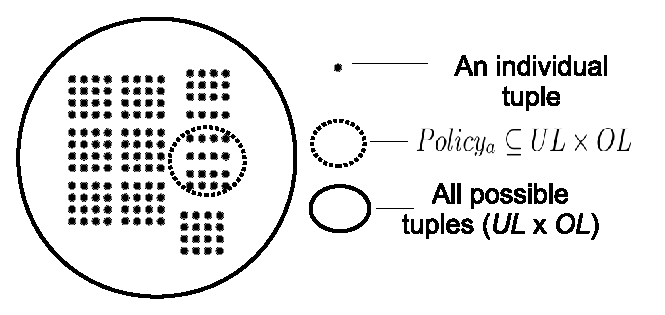
\includegraphics[width=.4\textwidth]{ABAC16/tuples-vs-policy}
 		\caption{Combining subset of tuples in a policy}
 		\label{fig:policy-vs-tuples}
 	\end{figure}
\begin{table}
\centering
\caption{Authorization policy space in \labacOneOneOne{}}
\label{tab:policy-enumeration}
\begin{tabular}{|l|l|}
\hline
\textbf{Item}                                           & \textbf{Size}               \\ \hline
Authorization policies                   & $ |A|$                       \\ \hline
Ways to define an Auth. policy       & $2^ {|UL| \times |OL|}$             \\ \hline
Ways to define all Auth. policies & $  |A| \times 2^{|UL| \times |OL|}$ \\ \hline
\end{tabular}
\end{table}


\chapter{EAP-ABAC vs LAP-ABAC in expressive power}

\chapter{Enforcement of \eapABAC{} models.}

\section{Enforcement in OpenStack Swift}
\section{Enforcement for JSON data}

\section{Conclusion \& Future work}
\label{sec:conclusion}


In this paper, we present a simple Attribute Based Access Control model (LaBAC) using enumerated policies. LaBAC is based on single user attribute ($\uLabel$) and single object attribute ($\oLabel$). We analyze LaBAC with other enumerated policy models. LaBAC can be viewed as a simple instance of an existing enumerated policy model - Policy Machine. LaBAC is also equivalent to \twoSortedRBAC{}, which is the other enumerated policy model as we are aware of. We show flexibility of LaBAC in terms of configuring traditional models (RBAC and LBAC) in it. 

Besides enumerated policy, we also discuss logical formula based authorization policy which is the more conventional approach for designing ABAC policy.  Logical formula can be very rich and complex and capable of expressing even complicated business logic in a very succinct form. But policy review or policy update may become NP-complete in policies expressed in logical formulas. 
%We believe, reviewing or updating policy would be  crucial in maintaining an ABAC system. This motivates us to explore other avenues in the design of an ABAC model. 

Enumerated policies as an alternate to specify authorization policies raise many interesting issues that need to be addressed to better  understand the nature of ABAC. For example, are there other alternates to specify authorization policies or policies in general in a ABAC system? What are the pros and cons of using logical formula or enumerated policy? Does review of policy or policy update become any simple in enumerated policies?  

Additionally, many other questions need to be addressed in term of enumerated policy ABAC models. Are enumerated policy models as expressive (or less/more) as logical formula based models? How (if possible) can we express arbitrary business logic in enumerated policies? What would be the cost of storing potentially large number of enumerated tuples? How can we extend LaBAC to incorporate more than one user and object labels (or attributes) and so on?

%On the contrary, enumerated policy is simple and policy review in it is inherently polynomial time. But there are many issues we need to be addressed in term of enumerated policy model. Is enumerated policy model less (or equal/more) expressive in general than logical formula based model?  Is there a  trade-off between expressive power and complexity of policy review/policy update? What would be the cost of storing potentially large number of enumerated polices? Are there alternates of designing ABAC policy other than or in between two extremes of logical formula and enumerated tuples and so on. 

%\section{Future work}



\appendix


\bibliographystyle{plain}
\nocite{*}
\bibliography{references}

\begin{vita}
	Prosunjit Biswas was born in Jessore, Bangladesh in 1984. Following his completion of secondary and higher secondary education from Jessore, Prosunjit received his Bachelor in Science (BS) degree in Computer Science from University of Dhaka, Bangladesh in 2008. He worked as a Software Developer in Bangladesh for 3 years. In 2011, he Joined UTSA to pursue his doctoral degree. He joined Institute for Cyber Security in 2012. His research interest is Attribute Based Access Control (ABAC). In particular, he is interested in developing flexible and administrative friendly models for ABAC.
	
\end{vita}

\end{document}
